%"runningheads" enables:
%  - page number on page 2 onwards
%  - title/authors on even/odd pages
%This is good for other readers to enable proper archiving among other papers and pointing to content.
%Even if the title page states the title, when printed and stored in a folder, when blindly opening the folder, one could hit not the title page, but an arbitrary page. Therefore, it is good to have title printed on the pages, too.
%\documentclass[runningheads,a4paper]{llncs}
\documentclass[conference]{IEEEtran}

\usepackage{tikz}
\usepackage{pgfplots}
\usepackage[latin1]{inputenc}

\usepackage{url}
\usepackage{times}
\usepackage{graphicx}
\usepackage{amsmath}
\usepackage{amssymb}

\usepackage{latexsym}
\usepackage{enumerate}
\usepackage{color}
\usepackage{booktabs}

\usepackage{pifont}

%Even though `american`, `english` and `USenglish` are synonyms for babel package (according to https://tex.stackexchange.com/questions/12775/babel-english-american-usenglish), the llncs document class is prepared to avoid the overriding of certain names (such as "Abstract." -> "Abstract" or "Fig." -> "Figure") when using `english`, but not when using the other 2.
\usepackage[english]{babel}

%better font, similar to the default springer font
%cfr-lm is preferred over lmodern. Reasoning at http://tex.stackexchange.com/a/247543/9075
\usepackage[%
rm={oldstyle=false,proportional=true},%
sf={oldstyle=false,proportional=true},%
tt={oldstyle=false,proportional=true,variable=true},%
qt=false%
]{cfr-lm}
%
%if more space is needed, exchange cfr-lm by mathptmx
%\usepackage{mathptmx}

\usepackage{graphicx}

%extended enumerate, such as \begin{compactenum}
\usepackage{paralist}

%put figures inside a text
%\usepackage{picins}
%use
%\piccaptioninside
%\piccaption{...}
%\parpic[r]{\includegraphics ...}
%Text...

%Sorts the citations in the brackets
%It also allows \cite{refa, refb}. Otherwise, the document does not compile.
%  Error message: "White space in argument"
\usepackage{cite}

\usepackage[T1]{fontenc}

%for demonstration purposes only
\usepackage[math]{blindtext}

%for easy quotations: \enquote{text}
\usepackage{csquotes}

%enable margin kerning
\usepackage{microtype}

%tweak \url{...}
\usepackage{url}
\urlstyle{same}
%improve wrapping of URLs - hint by http://tex.stackexchange.com/a/10419/9075
\makeatletter
\g@addto@macro{\UrlBreaks}{\UrlOrds}
\makeatother
%nicer // - solution by http://tex.stackexchange.com/a/98470/9075
%DO NOT ACTIVATE -> prevents line breaks
%\makeatletter
%\def\Url@twoslashes{\mathchar`\/\@ifnextchar/{\kern-.2em}{}}
%\g@addto@macro\UrlSpecials{\do\/{\Url@twoslashes}}
%\makeatother

%diagonal lines in a table - http://tex.stackexchange.com/questions/17745/diagonal-lines-in-table-cell
%slashbox is not available in texlive (due to licensing) and also gives bad results. This, we use diagbox
%\usepackage{diagbox}

%required for pdfcomment later
\usepackage{xcolor}

% new packages BEFORE hyperref
% See also http://tex.stackexchange.com/questions/1863/which-packages-should-be-loaded-after-hyperref-instead-of-before

%enable hyperref without colors and without bookmarks
\usepackage[
%pdfauthor={},
%pdfsubject={},
%pdftitle={},
%pdfkeywords={},
bookmarks=false,
breaklinks=true,
colorlinks=true,
linkcolor=black,
citecolor=black,
urlcolor=black,
%pdfstartpage=19,
pdfpagelayout=SinglePage,
pdfstartview=Fit
]{hyperref}
%enables correct jumping to figures when referencing
\usepackage[all]{hypcap}

%enable nice comments
\usepackage{pdfcomment}
\newcommand{\commentontext}[2]{\colorbox{yellow!60}{#1}\pdfcomment[color={0.234 0.867 0.211},hoffset=-6pt,voffset=10pt,opacity=0.5]{#2}}
\newcommand{\commentatside}[1]{\pdfcomment[color={0.045 0.278 0.643},icon=Note]{#1}}

%compatibality with TODO package
\newcommand{\todo}[1]{\commentatside{#1}}

%enable \cref{...} and \Cref{...} instead of \ref: Type of reference included in the link
\usepackage[capitalise,nameinlink]{cleveref}
%Nice formats for \cref
\crefname{section}{Sect.}{Sect.}
\Crefname{section}{Section}{Sections}

\usepackage{xspace}
%\newcommand{\eg}{e.\,g.\xspace}
%\newcommand{\ie}{i.\,e.\xspace}
\newcommand{\eg}{e.\,g.,\ }
\newcommand{\ie}{i.\,e.,\ }

%introduce \powerset - hint by http://matheplanet.com/matheplanet/nuke/html/viewtopic.php?topic=136492&post_id=997377
\DeclareFontFamily{U}{MnSymbolC}{}
\DeclareSymbolFont{MnSyC}{U}{MnSymbolC}{m}{n}
\DeclareFontShape{U}{MnSymbolC}{m}{n}{
    <-6>  MnSymbolC5
   <6-7>  MnSymbolC6
   <7-8>  MnSymbolC7
   <8-9>  MnSymbolC8
   <9-10> MnSymbolC9
  <10-12> MnSymbolC10
  <12->   MnSymbolC12%
}{}
\DeclareMathSymbol{\powerset}{\mathord}{MnSyC}{180}

% correct bad hyphenation here
\hyphenation{op-tical net-works semi-conduc-tor}

\begin{document}

%Works on MiKTeX only
%hint by http://goemonx.blogspot.de/2012/01/pdflatex-ligaturen-und-copynpaste.html
%also http://tex.stackexchange.com/questions/4397/make-ligatures-in-linux-libertine-copyable-and-searchable
%This allows a copy'n'paste of the text from the paper
\input glyphtounicode.tex
\pdfgentounicode=1

\title{Privacy, Polarization, and Passage of Divisive Laws}
%If Title is too long, use \titlerunning
%\titlerunning{Short Title}

%Single insitute
%\author{Firstname Lastname \and Firstname Lastname}
%If there are too many authors, use \authorrunning
%\authorrunning{First Author et al.}
%\institute{Institute}

%Multiple insitutes
%Currently disabled
%
%\iffalse
%Multiple institutes are typeset as follows:
%\author{Anonymized Author(s)}
%\author{Benjamin Johnson \and Paul Laskowski}


\author{\IEEEauthorblockN{Benjamin Johnson}
\IEEEauthorblockA{\textit{Chair of Cyber Trust} \\
\textit{Technical University of Munich}\\
Munich, Germany \\
benjamin.johnson@tum.de}
\and
\IEEEauthorblockN{Paul Laskowski}
\IEEEauthorblockA{\textit{School of Information} \\
\textit{University of California, Berkeley}\\
Berkeley, California,  USA \\
paul@ischool.berkeley.edu}
}




%If there are too many authors, use \authorrunning
%\authorrunning{First Author et al.}

%\institute{Anonymized Institution(s)}
%\institute{
%Technical University of Munich\\
%\email{benjaminejohnson@gmail.com}\and
%UC Berkeley\\
%\email{paul@ischool.berkeley.edu}
%}
%\fi
			
\maketitle

\begin{abstract}
%!TEX root = paper.tex
%abstract.tex
%
Notions of privacy are particularly salient to marginalized groups of people, especially when they find themselves disproportionately affected by the enforcement of laws.  We use game theoretic modeling to explore the connections between privacy, polarization, and the divisiveness of laws.  Our framework is based on a population of citizens that may be more or less polarized.  A law is defined in terms of its effect on each citizen and must gain support from a majority in order to pass.  We define a notion of divisiveness which allows us to measure the extent to which a law disproportionately affects different groups of citizens.  Our framework allows us to explore four distinct notions of privacy, two that result from technological measures and two that emerge from legal theory.  We find that privacy can prevent the passage of certain divisive laws, but the effects depend strongly on which type of privacy is in use.


\end{abstract}

%\keywords{Privacy, Polarization, Law, Search, Marginalized Populations}


%!TEX root = paper.tex
%intro.tex
%

\section{Introduction}
\label{sec:intro}




In 2006, Utah police received an anonymous tip about drugs being sold out of a house in South Salt Lake. Detective Douglas Fackrell spent several hours surveilling the house in an unmarked car, but saw only modestly suspicious activity.  After a week, he stopped an individual, Edward Strieff, as he was exiting the house and asked for identification.  When he discovered that Strieff had an outstanding warrant for a minor traffic violation, Detective Fackrell proceeded to search him and found methamphetamine in Strieff's pockets.  

This event marked the start of a legal battle that reached the US Supreme Court last year.  Although a warrant generally provides adequate reason for a search, the police conceded that Fackrell did not have reasonable suspicion to detain Strieff in the first place.  The supreme court has long held that evidence gained in violation of the Fourth Amendment is inadmissible as evidence - the so-called exclusionary rule.  The case revolves around the extent to which the exclusionary rule protects the privacy of citizens when new information, such as an arrest warrant, arrives after an improper detainment.

Although the Supreme Court ultimately ruled against Strieff, the case reveals the extent to which our value of privacy is bound up in notions of power and polarization.  During oral argument in February, Justice Sonya Sotomayor posed the following question. 

\begin{quote}``What stops us from becoming a police state and just having the police stand on the corner down here and stop every person, ask them for identification, put it through, and if a warrant comes up, searching them?"
\end{quote}

At the heart of this argument is a recognition that privacy protects entire groups of people.  One doesn't have to have drugs in one's pocket to object to arbitrary searches by police.  Privacy places limitations on police power, affecting the playing field faced by all citizens.  Even when the vast majority of police officers abide by strict ethical standards, the prospect of running into a corrupt one remains threatening.  Furthermore, the ability to invade the privacy of citizens has been argued to increase incentives for governments to abuse their power.~\cite{laskowskigovernment}

Calls for privacy are particularly acute when a particular group is disadvantaged or marginalized.  In this case, the laws that police enforce may disproportionally affect the marginalized group.  A classic example is the disparity between sentences for powder cocaine, typically associated with rich white communities, and crack cocaine, which is associated with disadvantaged black communities.  Before the fair sentencing act of 2010, the weight of powder cocaine needed to trigger certain federal criminal penalties was 100 times greater than the weight of crack cocaine that would trigger the same penalties.  This disparity is said to be a significant factor behind the large number of African Americans that were sentenced for drug offenses.~\cite{beaver2009getting}

To understand how laws and police enforcement affect disadvantaged groups, we must also understand how society is polarized between different groups of people to begin with.  How are laws passed that benefit one group at the expense of another group?  Moreover, can privacy protection help marginalized groups overcome their disadvantageous position?

In this paper, we use game theoretic modeling to explore the connections between privacy, polarization, and the passage of divisive laws.  Our framework is based on a population of citizens that influence what laws are passed, or what laws are maintained.  A law is defined in terms of how it impacts each individual, and our model is flexible in that it allows any set of effects.  We define a notion of divisiveness which allows us to measure the extent to which a law disproportionately affects different groups of citizens.

Divisiveness is not the only factor to consider when evaluating laws.  A divisive law may still be justified if it significantly improves welfare.  Progressive taxation is one example in which a law targets groups differently with the frequent aim of enhancing welfare.  On the other hand, some laws may not be divisive at all, but may still be welfare-decreasing or unjust for other reasons.  Nevertheless, we believe that divisiveness should generally be viewed as a cause for concern, especially when a law targets a marginalized group.

Our framework allows citizens to form opinions based on how a law impacts them directly, but it optionally allows them to consider the impact on others as well.  This is achieved through an influence matrix that is multiplied by the direct effect of the law.  This can be used to represent a concern for friends, loyalty to a larger group, or learning from a small number of influential personalities.  The influence matrix also allows us to discuss how polarized society is.  At the end of our analysis, we apply this framework to model a society with one majority group and one minority group.

Our model assumes that laws that are supported by a majority of citizens are passed or maintained.  Although the democratic process is generally much more complicated than a simple majority vote, we believe this is a useful and tractable way to explain the types of laws that exist in society.

Using our model of how laws are enforced, we are able to identity four distinct notions of privacy.  Two of these are technological, including strategies that citizens can take to hide features and behaviors from authorities.  The other two are legal notions, depending on a judicial branch that functions as a check on enforcement procedures. %police behavior. 
We describe the function of each of these privacy notions using our two-population model of society.  We find that each type of privacy allows a different set of laws to be passed and enforced, resulting in different effects on divisiveness.  Our work supports the idea that privacy, while far from a perfect cure, has a role to play in mitigating the divisive effects of laws in a society.

%Discussion examples
%\begin{itemize}
%\item Fergeuson style searches
%\item stop and frisk
%\item prohibition
%\item iphone data
%\item Muslim databases
%\end{itemize}



%!TEX root = paper.tex
%related.tex

\section{Related work}
\label{sec:related}

\subsection{Privacy and Government}
This work falls within a line of research that investigates the balance of power between citizens and the state. In~\cite{laskowskigovernment}, we investigated the application of surveillance technology by a government that wishes to remain in power.  Our main takeaway was that enhanced surveillance technology increases incentives for abuse. 

In a similar vein, Goh provides a model of a government that may employ surveillance to lower the risk of a terrorist attack \cite{goh2015prosperity}.  Greater surveillance carries an increased risk that citizens will learn of its existence, which increases the risk that the government loses power.  Goh finds that a rational government will employ less surveillance when citizens value their privacy more, but autocratic governments will employ more surveillance than democratic ones.

A larger literature examines the relationship between citizens and the state in general.  Downs~\cite{downs1957economic} provides a model of political competition based on a continuum of political preferences, extending Hoteling's study of horizontal differentiation~\cite{press39hotelling}.  Further studies model the process by which governments are overthrown.  Ginkel and Smith~\cite{ginkel1999so} consider factors that determine the probability of revolution in a repressive regime.  Lohmann~\cite{lohmann1994dynamics} describes the potential overthrow of a government through an informational cascade model. Kuran~\cite{kuran1989sparks} attempts to explain why revolutions often take the world by surprise with a game theoretic model of political change.  These studies do not consider the effects of privacy in determining political outcomes.

\subsection{Privacy and Firms}

Privacy also affects the relationship between citizens and firms, and several strands of research shed light on this topic (Acquisti provides a survey \cite{acquisti2010economics}).  Privacy can be seen in the classic literature on information economics as an information imbalance between a principal and an agent.  Moral hazard models assume that an agent's actions are not directly observable and the focus is on aligning incentives through contracting \cite{holmstrom1979moral}\cite{stiglitz1981credit}.  In models of adverse selection, agent types are private and certain types are driven out of a market because the principal cannot distinguish between them \cite{akerlof1995market}.  In signaling games, agents may engage in costly actions to signal their private type for economic gain \cite{spence1973job}.  None of these settings correspond to our focus on privacy as protecting a marginalized group.  Furthermore, models in this literature are usually neoclassical in the sense that privacy is an obstacle to maximizing welfare. 

An emerging body of privacy research models the behavior of consumers that participate in two different markets in sequence.  Firms in one market learn about consumers based on their purchase decisions and may be allowed to sell this information to firms in the second market.  A common theme in this literature is the fact that outcomes depend on whether consumers are myopic, considering each purchase decision without regard for how it will affect future purchases, or fully sophisticated.  In \cite{johnsoncaviar}, we found that when consumers are myopic, firms benefit greatly, but consumer surplus is also reduced. When we assume that consumers are strategic, consumers are better off, but firms fare worse.  In a similar vein, Acquisti and Varian look at a single monopolist that sells two goods in series \cite{acquisti2005conditioning}.  Taylor examines the case of two firms when consumer valuations for each good can take on two values, but these valuations are not perfectly correlated with each other \cite{taylor2004consumer}.  Information sharing may increase or decrease consumer surplus and welfare, depending on the demand specification.  

Other studies provide further examples of scenarios in which privacy is welfare-enhancing.  Hermalin and Katz discuss insurance markets and investments in information gathering \cite{hermalin2006privacy}.  Taylor considers a scenario in which collecting information about customers is costly and firms may overinvest in this activity \cite{taylor2003privacy}.  Hann et al. argue that unsolicited marketing imposes negative costs on consumers in the absence of privacy regulation \cite{hann2008consumer}.

A final literature studies privacy through the lens of mechanism design.  Calzolari and Pavan describe a framework in which firms may offer arbitrary contracts to users \cite{calzolari2006optimality}.   A set of recent papers have pioneered the use of differential privacy as a solution concept \cite{pai2013privacy}.  In these models, agents must be approximately truthful to the mechanism and cannot change the outcome by very much if they lie or refuse to participate.  Protecting privacy is not the focus of these models, since the solution concept begins with an assumption that agents don't hide information.

In contrast to the studies we mention, which treat privacy as a binary parameter, our work distinguishes four distinct types of privacy, which are inspired by technologies and legal debate.  We further apply our model to explore the effects of privacy on divisive laws.

\subsection{Technological Features of Privacy}

Citizens that engage in behavior that is forbidden by a law may employ privacy-enhancing technologies, such as the anonymizing Tor network~\cite{dingledine2003privacy}.  Sweeney defines a notion, k-anonymity, to measure the anonymity provided by a particular dataset \cite{sweeney2002k}. Technologies also mediate the enforcement of laws.  The ability of a government to identify law-breakers is enhanced through techniques like dataset aggregation\cite{acquisti2009predicting}.  An ongoing debate surrounds the use of these and other technologies, in contexts ranging from ethics\cite{lyon2002surveillance,diffie2010privacy}, to law\cite{landau2009,landau2013making,landau2014,Bankston14}, to security-relevant effectiveness~\cite{schneier2013oppression%,schneier2013surveillance
}.  While our model abstracts from these details, we will use it to explore the impact of technologically-based privacy.


\subsection{Polarization}
Most voters in the United States are overwhelmingly moderate in their policy positions\cite{layman2006party}.   Nevertheless, the United States Congress has passed a number of divisive laws, many of which have been challenged and overturned by the US Supreme Court.  Divisive laws have also been passed in European countries, including those against face covering, pejoratively dubbed ``burka bans.''


\begin{figure}[htbp]
\begin{center}
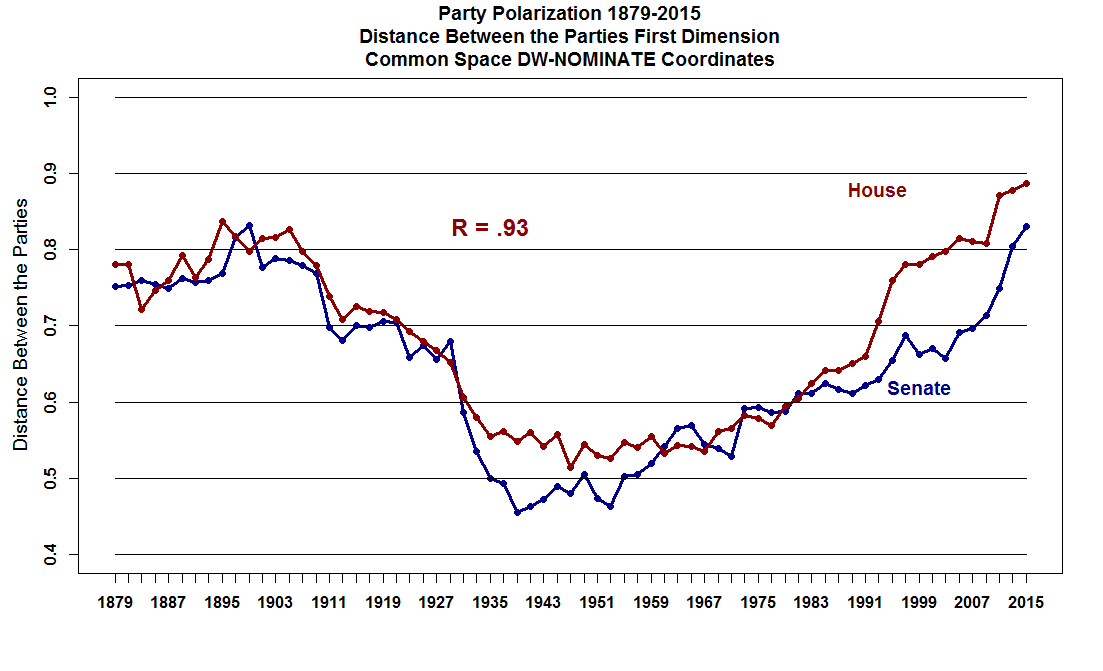
\includegraphics[width=0.4\textwidth]{figs/polar_house_and_senate_46-115_july_11}
\caption{{\bf Polarization Trends in the US Congress}}
\label{fig:uscongress}
\end{center}
\end{figure}




The United States congress in particular has become increasingly polarized over the last 40 years (see Figure \ref{fig:uscongress}).  Today, members of congress exhibit a distinctly bimodal distribution in terms of political preferences, as seen in \ref{fig:partisonship}.  Researchers have posited a number of reasons for this phenomenon \cite{barber2015causes}\cite{poole1984polarization}, ranging from a polarized electorate, to southern realignment, to gerrymandering, to the evolution of modern primary elections, to economic inequality, to money in politics, to the media environment, or to congress-based factors such as congressional rule changes, majority party agenda control, party pressures, teamsmanship, or the breakdown of bipartisan norms.  All of these issues are discussed in~\cite{poole1984polarization}.
More culturally-specific theories involving authoritarianism are also prevalent \cite{hetherington2009authoritarianism}.

\begin{figure}[htbp]
\begin{center}
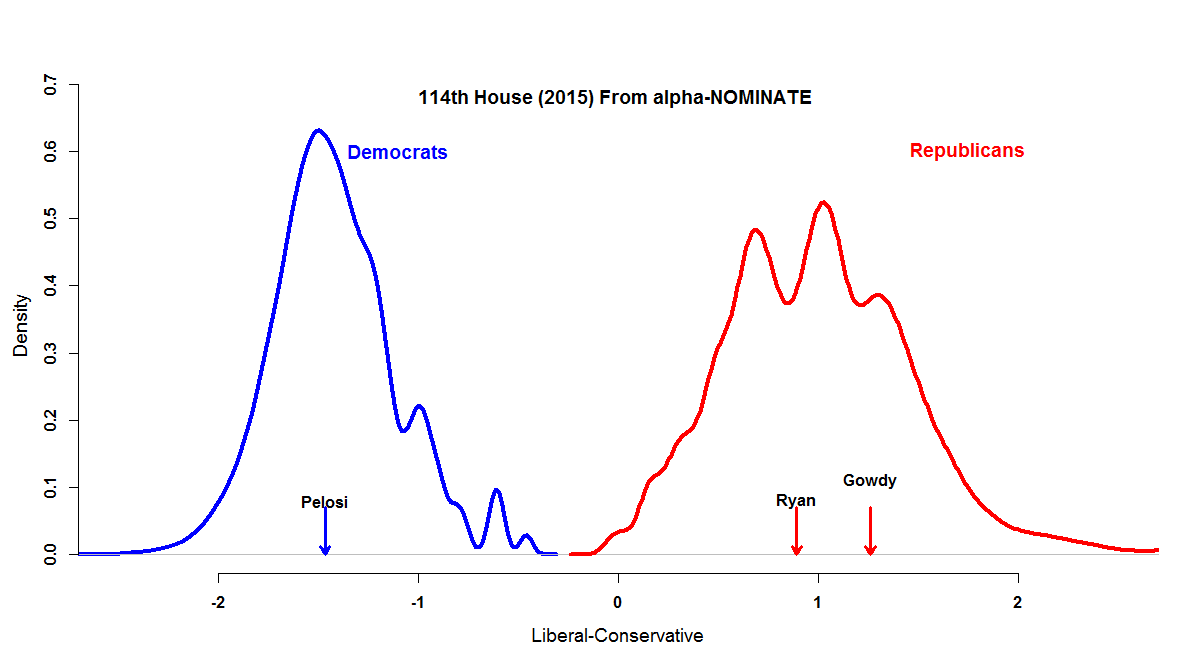
\includegraphics[width=0.4\textwidth]{figs/alpha_House_114_Histogram_8_January_2016}
\caption{{\bf Partisonship in the US House of Representatives}}
\label{fig:partisonship}
\end{center}
\end{figure}


%; and there is a remarkably close correlation between economic
%inequality and polarization in the United States~\cite{mccarty2006polarized}.  See Figure \ref{fig:inequality}.

%\begin{figure}[htbp]
%\begin{center}
%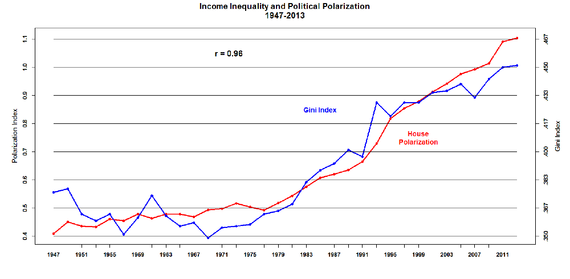
\includegraphics[width=0.4\textwidth]{figs/8141eb7a0}
%\caption{{\bf Polarization versus Income Inequality}}
%\label{fig:inequality}
%\end{center}
%\end{figure}


A more economically-driven explanation derives from the notion of information cascades. An information cascade occurs when people receive a noisy informational signal and observe the behavior of friends and colleagues to inform decision-making.  Although agents are individually rational, they may find it optimal to rely on the information they derive from previous agents, ignoring their private signals \cite{bikhchandani1992theory}.

The notion that people exhibit herding behavior in predictable circumstances has been around for decades \cite{shiller1995conversation}.  For example, researchers at Iowa State University conducted 259 interviews with farmers who had largely refused offers to adopt drought-resistant seed corn during the Great Depression and Dust Bowl.  They found that the slow rate of adoption was due to ``how farmers valued the opinion of their friends and neighbors instead of the word of a salesman''\cite{beal1957diffusion}.


We include a notion of influenced behavior in our model as a way to describe the polarization of society.  Our model does not mandate that citizens consider how a law affects other citizens, but merely allows it.  %This allowance appears justified by the observation that the United States has a legislative system that is organized like Figure \ref{fig:partisonship}, while it has an electorate that is more like Figure \ref{fig:voters}.




%
%\begin{figure}[htbp]
%\begin{center}
%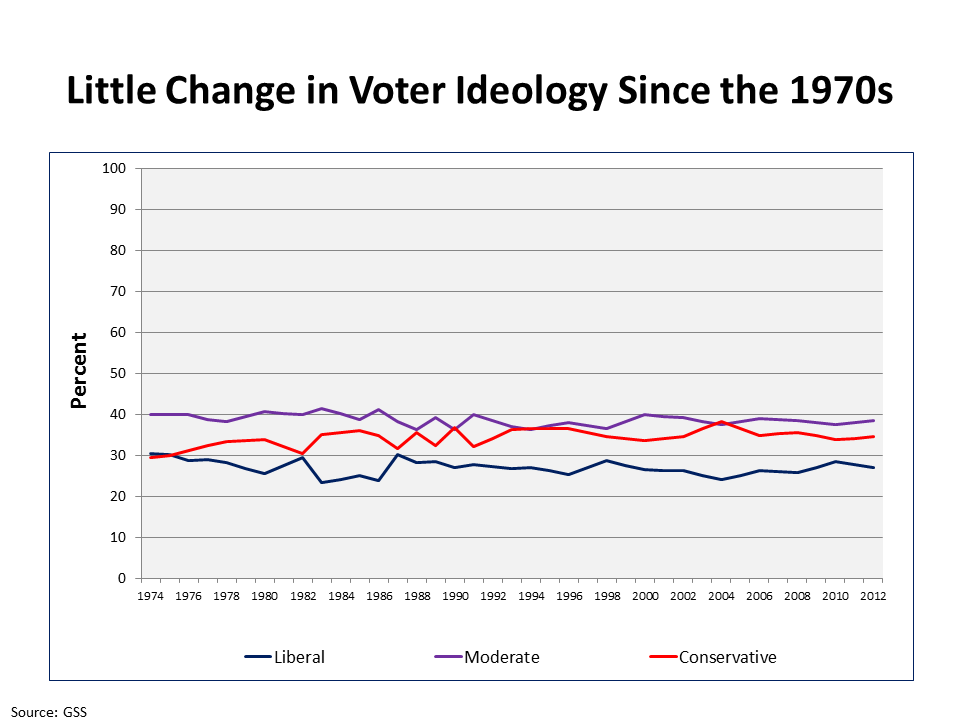
\includegraphics[width=0.4\textwidth]{figs/polarization2}
%\caption{{\bf Long Term Trends in US Voter Ideology}}
%\label{fig:voters}
%\end{center}
%\end{figure}
%





%!TEX root = paper.tex
%model.tex

\section{Model}
\label{sec:model} 


%\begin{tikzpicture}[scale = 6]
%
%       % x axis
%\draw [->] (0, 0) -- (1.1, 0) node [below right] {$P_0$};
%\draw [shift={(1.0, 0)}] (0,0.02) -- (0, -0.02) node[below] {$Cr(0)$};
%
%       % y axis
%\draw [->] (0, 0) -- (0, 1.3) node [above left] {$P_1$};
%\draw [shift={(0, 1.2)}] (-0.02,0) -- (0.02,0) node[shift={(-0.8,0)}] {$Cr(1)$};
%
%	%diagonal
%\draw [->,dashed] (-0.1, -0.1) -- (1.2, 1.2) node [above] {$B$};
%
%	%right
%\draw [-,dashed] (1, 0) -- (1, 1.2);
%
%	%top
%\draw [-,dashed] (0, 1.2) -- (1, 1.2); 
%
%	%point A
%\draw[shift={(0.2, 1.2)}] node [above] {$A$};
%
%\end{tikzpicture}

%
%\usetikzlibrary{patterns}
%
%\newcommand{\myaxes}{
%	\draw [->|] (0,0) node [left=1mm] {\scriptsize $$} -- node [rotate=90,above] {vertical label} (0,1.2) node [left=1mm,overlay] {\scriptsize $Cr(1)$};
%	\draw [->|] (0,0) node [below=1mm] {\scriptsize $0$} -- node [below] {horizontal label} (1,0) node [below=1mm] {\scriptsize $Cr(0)$};
%}
%
%\tikzstyle{full-protection}=[blue,pattern=north east lines,pattern color=blue];
%\tikzstyle{full-self}=[orange,pattern=north west lines,pattern color=orange];
%\tikzstyle{full-market}=[red,pattern=crosshatch dots,pattern color=red];
%
%\tikzstyle{partial-protection}=[blue,pattern=north east lines,pattern color=blue,opacity=.4];
%\tikzstyle{partial-self}=[orange,pattern=north west lines,pattern color=orange,opacity=.4];
%\tikzstyle{partial-market}=[red,pattern=crosshatch dots,pattern color=red,opacity=.4];
%
%\tikzstyle{partial-all}=[gray,pattern=grid,pattern color=gray,opacity=.4];
%
%\tikzstyle{passivity}=[dashed,thick];
%\tikzstyle{special}=[red,thick];
%
%\begin{tikzpicture}
%
%	%	Legend
%	
%%	\draw [special] (0,-.5) rectangle ++(.25,.25) ++(0,-.125) node [right=2mm,black,opacity=1] {partial protection and full market insurance};
%
%	\draw [partial-self,line width=.8mm,dash pattern=on 1mm off 1mm] (-.2,-.875)--++(.6,0) node [right=0mm,black,opacity=1] {area 6};
%	\draw [partial-market,line width=.8mm,dash pattern=on 1mm off 1mm] (.4,-.875)--++(-.6,0);
%
%	\draw [partial-protection,line width=.6mm] (-.2,-1.375)--++(.6,0) node [right=0mm,black,opacity=1] {area 5};
%	
%	\draw [partial-all] (0,-.5) rectangle ++(.25,.25) ++(0,-.125) node [right=2mm,black,opacity=1] {area 4};
%	\draw [full-market] (0,0) rectangle ++(.25,.25) ++(0,-.125) node [right=2mm,black,opacity=1] {area 3};
%	\draw [full-self] (0,.5) rectangle ++(.25,.25) ++(0,-.125) node [right=2mm,black,opacity=1] {area 2};
%	\draw [full-protection] (0,1) rectangle ++(.25,.25) ++(0,-.125) node [right=2mm,black,opacity=1] {area 1};
%\end{tikzpicture}
%
%\begin{tikzpicture}[>=stealth,scale=7]
%
%%	\draw [partial-all,draw=none] (.125,0) rectangle (1,.5);
%%	\draw [full-self,draw=none] (0,0)--(0,.375)--(.625,.375)--(1,0)--(0,0);
%%	\draw [full-protection,draw=none] (0,0) -- (.125,.125) -- (.125,1) -- (0,1) -- (0,0);
%%	% \draw [full-market,draw=none] (.125,.5) rectangle (1,1);
%%	\draw [full-market,draw=none] (0,.5) rectangle (1,1); % combined (1) and (5)
%%	
%%	\draw [partial-market,line width=.8mm,dash pattern=on 1mm off 1mm] (.5,.5) node [below,black] {\small FIX ME}--(1,.5);
%%	\draw [partial-self,line width=.8mm,dash pattern=on 1mm off 1mm] (1,.5)--(.5,.5);
%%	
%%	\draw [partial-protection,line width=.6mm] (.125,.5)--(.125,1);
%	
%%	\draw [special] (0,0) -- (.5,.5) -- (0,.5) -- (0,0);
%	\myaxes{}
%\end{tikzpicture}


\subsection{Definitions}
As we use the terms divisiveness, polarization, and privacy throughout the paper, we take care to define them here.

\begin{itemize}
\item  \emph{Divisiveness} of a law refers to the extent to which the different citizens value the law differently -- measured, for example, by the standard deviation in valuations.

\item \emph{Polarization} of a society refers to the grouping of individuals into sets that have little influence over each other, or that prioritize the welfare of insiders over that of outsiders.

\item \emph{Privacy} refers to an individual's ability to possess property (physical or intellectual) that is free from inspection or search. 

\end{itemize}

\subsection{Overview}
Our general model presents an incentive structure that relates the polarization of a society to the passage of divisive laws. Given a specific law, our model assumes the following. 
\begin{itemize}
\item Each individual begins with an initial evaluation of the law. We refer to this initial evaluation as the direct benefit for that individual.
\item Each individual's support for a law may (but need not) be influenced by other individuals.
\item Individuals are heterogeneous in their influence over others.
%\item Each individual may have a non-commutative influence on another individual's evaluation.
%%\item We distinguish an individual's derived benefit of a law from an individual's support of a law. 
%\item An individual's support is a function of their derived benefit together with a weighted influence of others. %influence With respect to a fixed law, suppose the mixing process happens and we measure, then we cannot tell the difference between the influence and the case where each individual makes their own evaluation or is influenced by others.  
\end{itemize}

%Want to talk about privacy.
\subsection {Citizen Influence}
For each pair of citizens $$i,j\in\{1,\dots N\},$$ define $$a_{ij}\in [0,1]$$ to be the influence of person $j$ on person $i$.  We may think of $a_{ij}$ also as the affinity person $i$ has toward person $j$. 

% into account when making decisions, or the extent to which person $j$ influences the decision of person $i$. 

Each individual will arrive at a level of support for the law based on a weighted average of the valuations of their influences, where the weighting is determined by the influence parameters $a_{ij}$. To be consistent with the notion of weighted average, we thus require $$\sum_ja_{ij}=1.$$%something similarly concrete-ish.

\subsection{Citizen Valuations of Laws}
Given a law $L$ and a citizen $j\in\{1,\dots N\}$, %define $$L(j)\in[0,1]$$ to be the probability that the law targets $j$.
%Alternatively, 
let $$V_L(i)\in\mathbb{R}$$ represent the direct impact of the law on person $i$. We assume that the direct impact of $L$ is unbounded because laws may save a life or take away life from individuals impacted by them.

If an individual's direct valuation for a law is perfectly in tune with the direct impact on the law then this person's support for a law will be $V_L(i)$. % weight his or her own opinion so much above others that for all practical purposes we have $a_{ii}\approx 1$, $a_{ij}\approx 0$ for $j\neq i$, and the support of $i$ for $L$ is exactly $$a_{ii}L(i)=L(i).$$
In other cases, for example where a law has little or no direct impact on the individual, a ban on muslims for example, initial evaluation of the law may be something very close to zero, i.e. neither positive nor negative.  Nevertheless a person's view of the law may evolve based on the views and experiences of their influences.  In such cases, we may suppose that after some amount of time, an individual's support for L evolves to become $$U_L(i)=\sum_ja_{ij}V_L(j).$$


%If we order the elements of this vector and graph it on a line, we can see directly from the graph a number of things
%\begin{enumerate}
%\item what percentage supports the law -- aka where the graph crosses the horizontal axis
%\item the existence of distinct homogeneous clusters -- regions along the horizontal axis where the function takes on a homogeneous value
%\item the extent to which the law is divisive for the society -- aka the magnitude of disutility for non-supporters of the law.
%\end{enumerate}
%
%How does privacy enter this picture?
%Privacy decreases the law's overall enforceability, and in particular, it makes it harder to enforce the law selectively.
%
%The crux of the analysis will be to show that privacy is especially welfare-enhancing in cases where a society is more polarized.
%!TEX root = paper.tex
%analysis.tex

\section{Analysis}
\label{sec:analysis}



\subsection{A Law Valuation Functional Form}
In this section, we specify a functional form for $V_L$ in order to discuss the effects of privacy.  While this reduces the generality of our model, it allows us to distinguish between different notions of privacy protection.  

We imagine that three conditions must apply for citizen $i$ to be punished by a law:

\begin{enumerate}
\item As the text of the law is written, it specifies that citizen $i$ is engaged in unlawful behavior.  We assume this occurs with probability $C(i)$.
\item Citizen $i$ is searched by the authorities.  We assume this occurs with probability $S(i)$.
\item A search on citizen $i$ is successful in finding evidence.  Conditional on the previous conditions, we assume this occurs with probability $F(i)$.  For simplicity, we will assume this function is a constant and write it as $F$.
\end{enumerate}

The probability that citizen $i$ is punished is therefore $S(i)C(i)F$. 
Let $P$ be the punishment for violating the law. Then each citizen's individual utility based only on the law's expected punishment on them may be given by 
$$S(i)C(i)F\cdot P.$$

We may also compute the total number of citizens punished by the law as $$\sum_j S(j)C(j)F.$$  

As far as the benefits of a law go, we assume that each individual $i$ suffers a cost $l_i$ each time a particular crime is committed.  This may be interpreted to include direct effects (e.g. the individual is targeted by theft or violence) as well as indirect effects (e.g. the prevalence of a crime makes the individual feel less welcome in their community).  For the current analysis, we assume that the number of crimes is reduced by exactly the number of people punished.  In other words, we do not allow for deterrent effects.  If such effects exist, they may multiply the effects of each search, and they may cause non-linearities in the valuation functions.  We defer these interesting issues to a future analysis.

Given these assumptions, we can write the initial valuation of law $L$ to person $i$ as the difference between the benefit gained from less crime and the individual's expected punishment in case she breaks the law. That is,  

$$V_L(i) = l_i \sum_j S(j)C(j)F - S(i)C(i)F\cdot P$$

%Each citizen earns a benefit from the law, proportional to the number of people that are caught, but earns disutility P if she is punished.

\subsection{Four Types of Privacy}
Our valuation model allows us to compare four types of privacy, the first two of which are technological in nature, and the second  two of which are legal.

\subsubsection{Attribute Privacy}

Attribute privacy is the notion that a person can conceal personal characteristics, which authorities may use to identify them as someone likely to commit a crime. \emph{Attribute privacy serves to prevent targeted searches.}  An example in which the attributes of individuals are fully or nearly anonymized is the case in which users of TOR hide their online activities. We may model this type of privacy by stipulating that $S(i)$ is a constant.
$$S(i)=S$$
%In less extreme cases, we may place restrictions on $S(i)$.

For a given text of a law, which implicitly specifies for each citizen $i$ the probability with which they are a criminal with respect to the law, restrictions on $S(i)$ (the probability that a citizen is searched) may prevent a majority from emerging to support the law.  %This is a simple consequence of the fact that restrictions on $S(i)$ translate into restrictions on $L_0(i)$ and $L_1(i)$. 
 In practice, when individual-targeted searches are prevented, we may expect authorities to restrict searches to a minority of the population, thereby ensuring that $V_L(i)$ is positive for a majority of individuals.

In this case, the shape of $V_L$ is entirely determined by the distribution of criminal behavior. Thus the number of individuals that support the law depends only on $C(i)$ and how polarized society is.

\subsubsection{Search Privacy}

Search Privacy is the idea that a citizen may use technology to prevent the discovery of evidence in the event that she is searched.  We represent this as a decrease in the parameter, $F$, 
$$F<1$$
representing the chance that evidence is found when a citizen breaking the law is searched.  In our valuation model, $F$ appears in both the positive and negative components of $V_L$ so that it does not change the number of citizens supporting the law. 

Nevertheless, this type of privacy will affect welfare, scaling it towards zero.  Search privacy may therefore be welfare-benefitting in the case of divisive laws for which welfare is negative.

\subsubsection{Search Quantity Privacy}

Our first legal notion of privacy corresponds to the idea that searches should not be widespread in a society.  Commentary discussed in the introduction involving  the recent supreme court case Utah v. Strieff exemplifies this notion.
%This is exemplified by a recent case before the US supreme court, Utah v. Strieff.  This case revolves around the extent to which the Fourth Amendment restricts police from searching citizens.  Detective Douglas Fackrell stopped Edward Strieff outside a house he was surveilling and asked for identification.  When he discovered that Strieff had an outstanding warrant for a minor traffic violation, he proceeded to search him and found methamphetamine in Strieff's pockets.  According to the so-called exclusionary rule, evidence gained in violation of the Fourth Amendment is generally not permitted in court, but it is unclear whether the rule applies when a warrant is found after an improper detainment.  During oral argument, justice Sonya Sotomayor asked ``what stops us from becoming a police state and just having the police stand on the corner down here and stop every person, ask them for identification, put it through, and if a warrant comes up, searching them?"
%
%At the core of these arguments lies a notion that searches should be rare in society rather than widespread.  
We encode this notion of privacy in our valuation model by requiring that the fraction of citizens that are searched is less than some bound, 
\begin{align}
\frac{\sum_j S(j)}{n} < m
\end{align}

Laws that don't meet this requirement may be declared unenforceable.  Search Quantity Privacy prevents the enforcement of laws against a large fraction of a population.


\subsubsection{Search Specificity Privacy}

Another notion of privacy supposes that authorities must have individualized reasonable suspicion to conduct a search.  This is similar to the notion of Search Quantity Privacy, defined above, but the focus is not on the total proportion of searches with respect to a population, but rather on how well-targeted the searches are.  We may encode this notion of privacy by requiring that a certain fraction of searches result in the finding of evidence,
\begin{align}
\frac{\sum_j S(j)C(j)F}{\sum_j S(j)} > \rho
\end{align}



\subsection{A Two-Party Influence Framework}

To further explore issues of privacy, we will place additional structure on citizen affinity.  In this section, we analyze the special case that there are two types of citizens, labeled 0 and 1.  Type 0 citizens are assumed to form the majority with population $n_0$.  Type 1 citizens form the minority with population $n_1 < n_0$.  

Within each group, we assume that all citizens share identical opinions regarding laws applied to their own group, and they also share identical opinions on laws applied to group outsiders. 
 %have identical influenced preferences.  That is, $U_L$ is constant in each group.  

For example, one way for this to happen would be if the influence function $a_{ij}$ itself were constant within each of the four cases $i,j<n_0$; $i<n_0,j\geq n_0$; $i\geq n_0,j < n_0$; and $i,j\geq n_0$. In this case, regardless of any individual's initial valuation of a law, the resulting final support for the law would be uniform within each group.  

As another example, we could assume that each of the two subgroups of citizens included a single influential thought leader, labeled $t_0$ and $t_1$.   
but decided on their support for the law on the exclusive basis of an aggregation of valuations from exactly two individuals labeled $i$ and $j$.  Citizens aligned with both $i$ and $j$ would have one valuation.  Citizens aligned with $i$ but not $j$ would have another, and so forth.  In terms of eventual support of a law, this scenario is indistinguishable from the example above.

%ese two scenAs in the previous case, regardless of individuals' initial valuations of the law, they would conform to $V_L(i)$at a fundamental experimental level, we e affinity of a citizen of type $i$ for a citizen of type $j$ is labeled $a_{ij}$.  For exposition, we make the additional assumption that 

For the sake of example, we will use the notations $a_{00}$ to represent the average affinity of an individual in the majority to the majority position.  We use $a_{01}$ to represent a majority individual's affinity for a minority person, and so forth for the other cases.  

Our only additional assumption is rather benign.  We assume that each group has a higher inter-group affinity than a cross-group affinity.  That is, 
%$a_{00} > a_{01}$ and $a_{11} > a_{10}$, meaning that citizens care more about what happens to an individual of their own type than one of the other type.  This also implies that 
\begin{align} 
a_{00} > \frac{1}{N}=\frac{1}{n_0+n_1} > a_{01} \\
a_{11} > \frac{1}{N}=\frac{1}{n_0+n_1}>  a_{10}
\end{align}

Given a law $(C, S, F)$, let $p_0 = C(0)S(0)F$ be the fraction of the majority that are punished, and let $p_1 = C(1)S(1)F$ be the fraction of the minority that are punished.  We use Figure~\ref{fig:criminals} to plot these quantities for different possible laws.  On this graph, the x-axis represents $p_0$ and the y-axis represents $p_1$.  In our model, the text of the law specifies the maximum fraction of each type of citizen that can be punished, $C(0)$ and $C(1)$, which occurs when $F=1$ and everyone is searched.  This region is represented by the outermost rectangle in the Figure, labeled A.



\begin{figure}[htbp]
\begin{center}


\begin{tikzpicture}[scale = 6]

       % x axis
\draw [->] (0, 0) -- (1.1, 0) node [below right] {$p_0$};
\draw [shift={(1.0, 0)}] (0,0.02) -- (0, -0.02) node[below] {$C(0)$};

       % y axis
\draw [->] (0, 0) -- (0, 1.3) node [above left] {$p_1$};
\draw [shift={(0, 1.2)}] (-0.02,0) -- (0.02,0) node[shift={(-0.8,0)}] {$C(1)$};

	%diagonal
\draw [->,dashed] (-0.1, -0.1) -- (1.2, 1.1) node [above] {$B$};

	%attribute privacy line 
\draw [->,dashed] (0, 0) -- (1.1, 1.32) node [above] {$C$};

	%right
\draw [-,dashed] (1, 0) -- (1, 1.2);

	%top
\draw [-,dashed] (0, 1.2) -- (1, 1.2); 

	%point A
\draw[shift={(0.2, 1.2)}] node [above] {$A$};

	%right of search privacy
\draw [-,dashed] (.5, 0) -- (.5, .6);

	%top of search privacy
\draw [-,dashed] (0, .6) -- (.5, .6); 

	%point D
\draw[shift={(0.35, .6)}] node [above] {$D$};

	%top of search quantity privacy
\draw [-,dashed] (0, .85) -- (.6, 0); 

	%point E
\draw[shift={(0.1, .75)}] node [above] {$E$};


\end{tikzpicture}
\caption{This figure shows the effects of privacy on divisive laws.}
\label{fig:criminals}
\end{center}
\end{figure}


Since more than half of the population is of type 0, a law may pass whenever the support of each type-0 individual is nonnegative.  We may compute support from individuals of type 0 as follows,

\begin{align}
U_L(i)&(0) = n_0 a_{00}  V_L(0) + n_1 a_{01}  V_L(1) \\
&= \beta t - n_0 a_{00}p_0 P - n_1 a_{01}  p_1 P \\
&= \beta \left[ \frac{n_0 p_0}{n_0 + n_1}   + \frac{n_1 p_1}{n_0 + n_1} \right]  - n_0 a_{00}p_0 P - n_1 a_{01}  p_1 P \\
&= \left[  \frac{\beta n_0}{n_0 + n_1} - n_0 a_{00}P  \right]p_0 + \left[ \frac{\beta n_1}{n_0 + n_1} -  n_1 a_{01}P \right] p_1
\end{align}

Letting $b_{00} = \frac{\beta }{n_0 + n_1} -  a_{00}P $ and $b_{01} = \frac{\beta}{n_0 + n_1} -   a_{01}P $, we can write,

\begin{align}
U_L(0) = b_{00}n_0p_0 + b_{01} n_1p_1 
\end{align}

Our assumption that $a_{00} > a_{01}$ guarantees that $b_{00} < b_{01}$.  This means that there are 3 possibilities for the signs of the coefficients on $p_0$ and $p_1$.

\begin{enumerate}
\item $\partial U_L(0) / \partial p_0 \leq 0$ and $\partial U_L(0) / \partial p_1 \leq 0$.  This will happen whenever $\beta \leq   a_{01}P(n_0 + n_1)  $, meaning that the benefit from the law is small relative to the size of the punishment multiplied by the affinity of the majority for the minority.
\item $\partial U_L(0) / \partial p_0 \leq 0$ and $\partial U_L(0) / \partial p_1 > 0$.  This will happen whenever $  a_{01}P(n_0 + n_1) < \beta  \leq a_{00}P(n_0 + n_1) $, or for intermediary amounts of benefit.  In this case, the majority will tend to support laws that punish the minority more and the majority less.
\item $\partial U_L(0) / \partial p_0 > 0$ and $\partial U_L(0) / \partial p_1 > 0$.  This will happen whenever $   a_{00}P(n_0 + n_1) < \beta$, or for high amounts of benefit.  In this case, the majority will tend to support laws that punish both groups as much as possible.
\end{enumerate}

The middle possibility, in which majority support increases with $p_1$ but decreases with $p_0$ is of particular interest, since this is the case in which the majority would favor the most divisive treatment of the two groups.

A law will have majority support if and only if $U_L(0) \geq 0$.  This can be written as,

\begin{align}
U_L(0) = b_{00}n_0p_0 + b_{01} n_1p_1 \geq 0
\end{align}

If condition 1 holds above, no law within rectangle A can have majority support, except for the origin.  This means that nobody will be punished and no benefit results.  If condition 3 holds above, every law within rectangle A has majority support, so a law may pass for any values of $S(0)$, $S(1)$, and $F$.  For the more interesting condition 2, the previous equation divides rectangle A into two regions.  This is depicted by line B in Figure \ref{fig:criminals}.  Every law that falls on this line or above can have majority support.

Using a similar argument to that above, we can derive the support of a type 1 citizen for the law to be

\begin{align}
U_L(1) =  b_{10} n_0p_0 + b_{11}n_1p_1
\end{align}

where $b_{10} = \frac{\beta}{n_0 + n_1} -   a_{10}P$ and $b_{11} = \frac{\beta }{n_0 + n_1} -  a_{11}P $ .  Since we assume $a_{10} < a_{11}$, we have $b_{10} > b_{11}$.

We compute divisiveness as the standard deviation,

\begin{align}
s_L &= \sqrt{var(U_L)}  =  \sqrt{E\left[ \left(U_L - \bar{U_L} \right)^2 \right] }  \\
&= \sqrt{ \frac{ n_0\left(U_L(0) - \bar{U_L}\right)^2 + n_1\left(U_L(1) - \bar{U_L} \right)^2 }{n_0+n_1}  }
\end{align}

where $\bar{U_L} = \frac{n_0 U_L(0) + n_1U_L(1) }{n_0 + n_1}$ is the average support for the law.  After some algebra, this can be simplified to the following,

\begin{align}
s_L &= \frac{\sqrt{n_0n_1}}{n_0 + n_1} \left| U_L(0) - U_L(1) \right|
\end{align}

In the region of laws that have majority support, it can be shows that $U_L(0) > U_L(1)$. Substituting for $U_L(0)$ and $U_L(1)$, we have

\begin{align}
s_L &= \frac{\sqrt{n_0n_1}}{n_0 + n_1} \left(  b_{00}n_0p_0 + b_{01} n_1p_1 - b_{10} n_0p_0 - b_{11}n_1p_1 \right) \\
&= \frac{\sqrt{n_0n_1}}{n_0 + n_1} \left(  ( b_{00} - b_{10} )n_0p_0 + ( b_{01} - b_{11})n_1p_1 \right) \\
&= \frac{\sqrt{n_0n_1}}{n_0 + n_1} \left(  ( a_{10} - a_{00} )P n_0p_0 + ( a_{11} - a_{01})P n_1p_1 \right) \\
\end{align}

by the ordering on our affinities, we know $a_{10} - a_{00}  < 0$ and $a_{11} - a_{01} > 0$ so

\begin{align}
\partial s_L / \partial p_0 <0 \\
\partial s_L / \partial p_1 >0
\end{align}

In other words, in the region of laws with majority support, divisiveness goes up with the number of minority members punished and down with the number of minority members punished.  This means that the law most favored by the majority, which is in the upper left corner of rectangle A, is also the most divisive.

\subsection{Privacy Effects}
Having outlined some basic properties of our model, we turn our attention to the effects of different types of privacy.  

\subsubsection{Effects of Attribute Privacy}
We begin with attribute privacy, which we understand to mean restrictions on S(0).  We model the extreme case of anonymity, represented as $S(0) = S(1)$.  The set of possible laws is represented by line C in Figure \ref{fig:criminals}.  Note that line C passes through the point $ \left(C(0), C(1) \right)$ at the upper right of rectangle A.  A more moderate version of attribute privacy may place bounds on the ratio of $S(1)$ to $S(0)$.  For example, we may specify,

\begin{align}
0 < \underbar r < S(1) /S(0) < \bar r < \infty
\end{align}

Since divisiveness is maximized at the point $ \left(0, C(1) \right)$, attribute privacy necessarily reduces the maximum amount of divisiveness since it disallows laws at this point.  As the figure is depicted, the slope of line C is greater than the slope of line B,

\begin{align}
C(1)/C(0) > - b_{00}n_0 / b_{01}n_1 
\end{align}

This means that any law that falls inside line C and rectangle A will also have majority support.  The majority would offer the most support to laws that fall further to the upper right of the line.  It is also possible, for the slope of line C to be less than the slope of line B,

\begin{align}
C(1)/C(0) > - b_{00}n_0 / b_{01}n_1 
\end{align}

In this case, no law on line C will have majority support except for a law at the origin.  Nevertheless, divisiveness decreases since having no law or a law at the origin brings divisiveness to zero.


\subsubsection{Effects of Search Privacy}

We interpret search privacy to mean that not all individuals who are searched while committing a crime are caught, 

\begin{align}
F<1
\end{align}

This condition limits the maximum number of people, of either type, who may be punished.  This is depicted by rectangle D in Figure \ref{fig:criminals}.  Like attribute privacy, search privacy reduces the maximum amount of divisiveness that can be caused by a law.  Specifically, the maximum divisiveness is reduced by a factor of F.  Unlike attribute privacy, search privacy never results in a scenario in which a previously enforced law can no longer have majority support.  As long as $S(0)$ and $S(1)$ are unchanged, reducing F still results in a law with majority support.  Divisiveness and welfare are simply scaled downwards.

\subsubsection{Effects of Search Quantity Privacy}

To model a policy of search quantity privacy, we impose the condition, 

\begin{align}
%\frac{\sum_j S(j)}{n_0 + n_1} = 
\frac{n_0 S(0) + n_1 S(1)}{n_0 + n_1}  < m
\end{align}

The maximum value of $S(0)$ can be attained when $S(1) = 0$, allowing $S(0) = m (n_0 + n_1)/n_0$.  Similarly, when $S(0) = 0$, $S(1)$ can attain a value of $S(1) = m (n_0 + n_1)/n_1$.   Note that the maximum value of $S(0)$ is smaller than the maximum value of $S(1)$.  This feature is plotted as line E in Figure \ref{fig:criminals}.  Laws below this line are acceptable under the search quantity standard.  

As the figure demonstrates, search quantity privacy may reduce the maximum possible divisiveness of a law.  The majority will still favor a law that is at the top corner of the acceptable region, which represents the maximum amount of divisiveness for a given amount of searches.  If the bound $m$ is not set low enough, the maximum amount of divisiveness may not be reduced at all.

\subsubsection{Effects of Search Specificity Privacy}

Search Specificity Privacy requires a certain proportion of searches to turn up evidence that an individual is breaking the law.  We represent this by writing,

$$\frac{\sum_j S(j)C(j)F}{\sum_j S(j)} = \frac{ n_0 S(0)C(0)F + n_1 S(1)C(1)F}{n_0 S(0) + n_1 S(1)}  > \rho$$

Rearranging,

\begin{align}
\nonumber n_0 S(0)C(0)F + n_1 S(1)C(1)F &> \rho n_0 S(0) + \rho n_1 S(1) \\
\nonumber  (n_1 C(1)F - \rho n_1 ) S(1) &>  - (n_0 C(0)F - \rho n_0 )S(0) \\
\end{align}

When $\rho$ is close enough to 0, the left hand side is nonnegative and the right hand side is nonpositive, so the constraint does not bind.  The set of possible laws is therefore not reduced.  On the other hand, when $\rho$ is close enough to 1, the left hand side is nonpositive and the right hand side is nonnegative, so the constraint binds unless $S(0) = S(1) = 0$.  No law can pass the privacy requirement except for the trivial one that doesn't punish anyone.  

The more interesting region is when $rho$ lies between  $C(0)F$ and $C(1)F$.  In the case that $C(1) > C(0)$, meaning that the text of the law targets behavior that is more common for individuals of type 1, we can write the constraint as,

\begin{align}
\frac{S(1)}{S(0)} &>  \frac{\rho n_0 - n_0 C(0)F }{n_1 C(1)F - \rho n_1}
\end{align}

where the fraction is arranged so that the numerator and denominator are positive.  This constraint is depicted by line F in Figure \ref{fig:criminals}.  Every law above this line is permitted under the search specificity rule.  Unfortunately, this rule does nothing to reduce the maximum possible divisiveness of a law.  In fact, it may have the opposite effect, allowing only laws for which members of the minority are much more likely to be searched than members of the majority.

In part, this conclusion may be the result of limitations of our model.  We have assumed that all members within a group have equal odds of breaking the law and equal odds of being searched.  A more detailed model might allow individuals to vary within each group.  Authorities may be able to select a smaller fraction of each group, choosing individuals with a higher probability of breaking the law, thereby increasing the proportion of searches that turn up evidence.  In such a model, search specificity privacy may be expected to limit the maximum divisiveness of a law.  Nevertheless, we believe that our central insight, that search specificity privacy limits searches on the majority more than on the minority, will continue to hold.







%!TEX root = paper.tex
%results.tex

%\section{Numerical Illustrations}
%\label{sec:results}
%



%
%The shaded region in Figure \ref{fig:surplus2} shows the total consumer surplus in equilibrium when $k=1$.
%
%\begin{figure}
%\begin{center}
%\includegraphics[width=0.75\textwidth]{plots/figure3}
%\caption{figure 3}
%\label{fig:surplus2}
%\end{center}
%\end{figure}
%

%%
% $Id: numerical.tex 686 2010-02-22 19:46:41Z nicolasc $
%
\section{Numerical evaluation}
\label{sec:numerical}

\begin{figure}
\begin{center}
\includegraphics[width=0.75\textwidth]{plots/gamma}
\caption{\label{fig:gamma} {\bf Gamma -- clever caption here.} Explanation of the clever caption.}
\end{center}
\end{figure}
\begin{figure}
\begin{center}
\includegraphics[width=0.75\textwidth]{plots/bs}
\caption{\label{fig:bs} {\bf Best shot.} Explanation of the clever caption.}
\end{center}
\end{figure}
\begin{figure}
\begin{center}
\shortstack{
        \includegraphics[width=0.75\textwidth]{plots/wl}\\
        {\footnotesize (a) Overall trends.}
}
\quad
\shortstack{
        \includegraphics[width=0.45\textwidth]{plots/wl2}\\
        {\footnotesize (b) Zoom on small values of the protection cost $b$.}
}
\caption{\label{fig:wl} {\bf Weakest link.} Explanation of the clever caption.}
\end{center}
\end{figure}
\begin{figure}
\begin{center}
\includegraphics[width=0.75\textwidth]{plots/te}
\caption{\label{fig:te} {\bf Total effort.} Explanation of the clever caption.}
\end{center}
\end{figure}

%!TEX root = paper.tex
%concl.tex

\section{Discussion and Conclusion}
\label{sec:concl}

Our study is an attempt to understand privacy, not at the level of individual incentives, but at the level of communities and the relationships they have to each other.  Though our modeling framework is exploratory, it reveals some of the complexity inherent in this setting.  We were able to relate privacy to polarization and the divisiveness of laws, but found that outcomes depend critically on what notion of privacy is in play.  Privacy enforced through technology can have dramatic effects on what laws are enforced, but all laws may be rendered ineffective whether divisive or not.  A privacy technology works equally well, after all, whether it is concealing sexual behavior between consenting adults, or a plot to assassinate a leader in government.  Legal notions of privacy hold the promise of more precise judgements.  Courts can identify disadvantaged groups and extend protections to them, without extending those same protections to say, serial killers.  Yet our model predicts that here too, privacy is not perfectly tailored to prevent the enforcement of divisive laws.  Further research is needed to assess how privacy laws may work in conjunction with anti-discrimination laws and policies, to better protect marginalized groups. 

In the future, we plan to extend our model to capture more features of the legal system and of privacy protection.  One important addition will be a description of how authorities gather information on potential law breakers.  A detailed model might describe citizens with a collection of attributes, each of which may carry information about a citizen's propensity to violate a specific law.  Some attributes may be hidden with technological privacy measures, some may be the topic of legal protection, and others may remain public and available to police as they direct their investigations.  

We would further like to model the issues that arise when police have the right to search a large number of people, but only enough resources to choose a small number.  The ability to arbitrarily select which citizens to search carries a significant amount of power, even when the number of searches remains small.  A more complete model would separate legality from the actual performance of a search in order to highlight these issues.

As technology advances, many established notions of privacy face considerable pressure to evolve.  Location monitoring, deep packet inspection, linking of consumer databases, and face recognition are just a few of the threats to our ability to control our personal information.  We hope that studies like ours will help spur discussion about the role privacy plays in maintaining balances of power, and how future definitions of privacy may best be structured to protect vulnerable groups and individuals.




%\subsubsection*{Acknowledgments}
%We thank ourselves for writing this paper.

%%%%%%%%%%%%%%%%%%%%%%%%%%%%%%%%%%%%%%%%%%%%%%%%%%%%%%%%%%%%%%%%%%%%%%%%%%%%%%%
\bibliographystyle{splncs03}
\bibliography{references}

%%%%%%%%%%%%%%%%%%%%%%%%%%%%%%%%%%%%%%%%%%%%%%%%%%%%%%%%%%%%%%%%%%%%%%%%%%%%%%%

\end{document}
